\documentclass[letterpaper]{article}
	
\usepackage{fullpage}
\usepackage{mathtools}
\usepackage{qtree}
\usepackage[section]{placeins}
\usepackage{subcaption}
\usepackage{float}
\DeclarePairedDelimiter{\ceil}{\lceil}{\rceil}
\DeclarePairedDelimiter{\floor}{\lfloor}{\rfloor}
{\renewcommand{\arraystretch}{1.2}
\usepackage{wrapfig}
\usepackage{changepage}  


\title{CS405G Mid-Project Report}

\author{Mati Turner, Matt Ruffner, Matt Dunbar}

\begin{document}
\maketitle

%%%%%%%%%%%%%%%%%%%%%%%%%%%%%%%
%%%%%%%%%%%%%%%%%%%%%%%%%%%%%%% GROUP INFO
%%%%%%%%%%%%%%%%%%%%%%%%%%%%%%%
\section{Group Information}
For the purposes of this document, team members will be referred to by their last names to avoid confusion.

The group for this project will consist of Mati Turner, Matt Ruffner and Matt Dunbar. All of us contributed to the creation and design of the database schema. We collaborated to find the simplest design that would allow for efficient queries while still supporting all necessary, and some extra, features.

Moving forward, Turner and Ruffner will focus on creating PHP pages to facilitate DB connection and querying, this will be known as the back-end. Ruffner and Dunbar will work on the user interface which will be constructed using Google's PolymerElements \footnote{https://www.polymer-project.org/1.0/}, this will be known as the front-end.

Data transfer between the front and back ends will be done using AJAX requests provided by the \texttt{iron-ajax} Polymer Element. \footnote{https://elements.polymer-project.org/elements/iron-ajax}

All group members will work on deciding a standardized data structure to be passed from the back to front when requests or actions are initiated, e.g. a search for items or user login.




%%%%%%%%%%%%%%%%%%%%%%%%%%%%%%%
%%%%%%%%%%%%%%%%%%%%%%%%%%%%%%% DB REQUIREMENTS AND SCHEMA
%%%%%%%%%%%%%%%%%%%%%%%%%%%%%%%
\section{Database Needs}
Our database will need the ability to:
\begin{itemize}

\item \textbf{Create tables} While it may only be once in the inception of our service, we will need to explicitly create tables to store our data.

\item \textbf{Insert data into tables}  Upon explicitly adding items or upon customer interaction, our database system will need to insert entries into the created tables following certain restraints.

\item \textbf{Update data in tables} Based on our following implementation of the prompt, updating entries within the tables will be crucial to our ordering process.  As such, our database will need to be able to access entries within a table and change the value of one or more of that entry’s attributes.

\item \textbf{Check statements to ensure referential integrity} For consistency’s sake, we will need to have access to Check statements to make sure no invalid data gets entered into the tables.

\item \textbf{Trigger statements} For sound design, it is important that the database have access to being triggered to warn for possible malicious or accidental input.

\end{itemize}
\hfill










%%%%%%%%%%%%%%%%%%%%%%%%%%%%%%%
%%%%%%%%%%%%%%%%%%%%%%%%%%%%%%% ER DIAGRAM
%%%%%%%%%%%%%%%%%%%%%%%%%%%%%%%
\section{ER Diagram}

\begin{figure}[H]
\centering
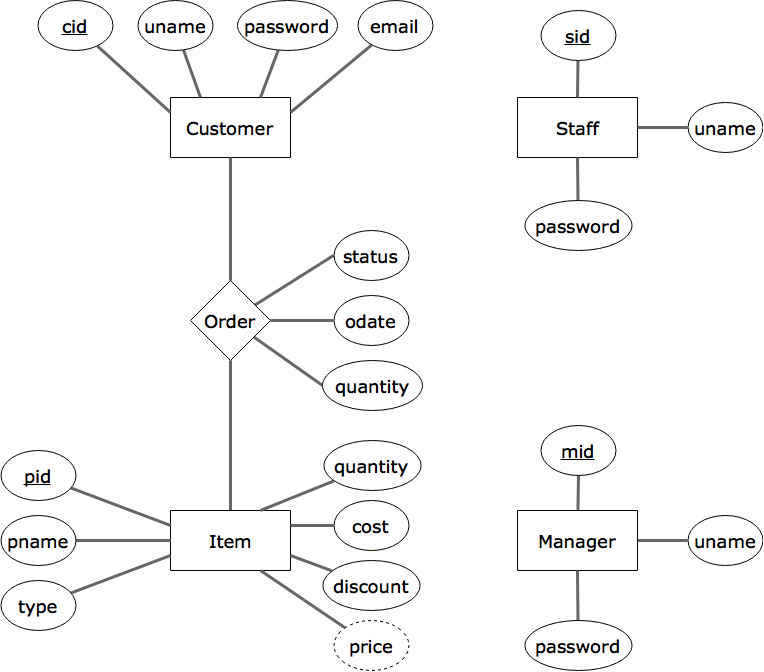
\includegraphics[width=\textwidth]{project-schema.png}
\end{figure}



\pagebreak
%%%%%%%%%%%%%%%%%%%%%%%%%%%%%%%
%%%%%%%%%%%%%%%%%%%%%%%%%%%%%%% DB REQUIREMENTS AND SCHEMA
%%%%%%%%%%%%%%%%%%%%%%%%%%%%%%%
\section{Database Schema Design}
%%%%%%%%%%%
%%%%%%%%%%% CUSTOMER TABLE
%%%%%%%%%%%
\textbf{Customer( primary key \textit{cid}: int, \textit{uname}: string, \textit{password}: string, \textit{email}: string)}
\begin{adjustwidth}{1.5cm}{}
The cid will be a number that will be assigned in the back-end by auto-incrementation.  (Each entry will make the cid be the next consecutive number starting at 0). The \textit{uname}, \textit{password} and \textit{email} are all given by the user.
\end{adjustwidth}\*\\
%%%%%%%%%%%
%%%%%%%%%%% STAFF TABLE
%%%%%%%%%%%
\textbf{Staff( primary key \textit{sid}: int, \textit{uname}: string, \textit{password}: string)}
\begin{adjustwidth}{1.5cm}{}
The \textit{sid} will be a number assigned in the back-end similar to the \textit{cid} for customers.  The \textit{uname} and \textit{password} will be set up either by the staff register or explicitly made for the purpose of testing the system.
\end{adjustwidth}\*\\
%%%%%%%%%%%
%%%%%%%%%%% MANAGER TABLE
%%%%%%%%%%%
\textbf{Manager( primary key \textit{mid}: int, \textit{uname}: string, \textit{password}: string)}
\begin{adjustwidth}{1.5cm}{}
The \textit{mid} will be a number assigned in the back-end similar to the \textit{cid} for customers.  The \textit{uname} and \textit{password} will be set up explicitly made for the purpose of testing the system.
\end{adjustwidth}\*\\
%%%%%%%%%%%
%%%%%%%%%%% MANAGER TABLE
%%%%%%%%%%%
\textbf{Item( primary key \textit{pid}: int, \textit{pname}: string, \textit{type}: string, \textit{cost}: real, \textit{discount}: real, \textit{price}: real, \textit{quantity}: int)}
\begin{adjustwidth}{1.5cm}{}
\textit{pid} will be a four-digit number much like the cid, mid, and sid of earlier relations.

\textit{pname} is the name of the item.

\textit{type} is “toy” or “game” (for sorting purposes).

\textit{cost} is a hidden value that is the raw cost of the item.  There will be a check on creation and update to ensure this is a positive value.

\textit{discount} is a real between 0 and 1 which signifies the discount on the item currently (set to 0 by default).  There will be a check on update to make sure that this value stays between 0 and 1 and there will probably be a confirmation check if a greater than 50\% discount was indeed intended.

\textit{price} is a derived quantity that is found from the following expression: cost-(discount)*cost

\textit{quantity} is pretty self explanatory.  There will be a check to make sure this value stays above zero in both creation and update.
\end{adjustwidth}\*\\
%%%%%%%%%%%
%%%%%%%%%%% ORDER TABLE
%%%%%%%%%%%
\textbf{Order( foreign key \textit{cid}: int, foreign key \textit{pid}: int, \textit{status}: string, \textit{quantity}: int, \textit{odate}: date)}
\begin{adjustwidth}{1.5cm}{}
The foreign keys \textit{cid} and \textit{pid} reference the tables Customers and Items.  There will be a check to ensure that these fall within the bounds of the current maxima and minima for these IDs (because they are consecutive in creation).

The string for \textit{status} will contain the values “pending”, “shipped”, or “cart”.  These refer to when an item has been bought, shipped, and put in a cart respectively.  When a user chooses to check out, the order will be updated from “cart” to “pending”.  When a staff member ships, the \textit{status} will update from “pending” to “shipped”.

The \textit{odate} is a time stamp specifying when the item was bought not carted.  This is done to ensure that items bought within the same cart will have the same \textit{odate}. This will also allow a user looking through their past orders to see them grouped by date and time.  When an item is carted the \textit{odate} will be NULL.
\end{adjustwidth}

\end{document}
